% !TEX root = ../Thesis.tex
%%
%%  Hochschule für Technik und Wirtschaft Berlin --  Abschlussarbeit
%%
%% Anhang
%%
%%%%%%%%%%%%%%%%%%%%%%%%%%%%%%%%%%%%%%%%%%%%%%%%%%%%%%%%%%%%%%%%%%%%%

\chapter{Anhang} \label{Anhang}

\section{Quelltext zur Datenaufbereitung}

Die folgenden Skripte wurden im Rahmen der Datenaufbereitung eingesetzt (siehe Abschnitt \ref{Konzept}) und sind aufgrund ihres Umfangs hier statt im Haupttext hinterlegt.

\begin{lstlisting}[caption=Code zur Umwandlung von .mp4 zu .png, label=lst:mp4topng]
import cv2
import os

video_path = "/home/oem/Desktop/BIldmaterial/IMG_0002.MOV"
output_dir = "extracted_images"
interval_seconds = 1

if not os.path.exists(output_dir):
    os.makedirs(output_dir)

cap = cv2.VideoCapture(video_path)
fps = cap.get(cv2.CAP_PROP_FPS)
interval_frames = int(fps * interval_seconds)

count = 0
image_id = 0

while cap.isOpened():
    ret, frame = cap.read()
    if not ret: break

    if count % interval_frames == 0:
        cv2.imwrite(f"{output_dir}/img_{image_id:04d}.png", frame)
        image_id += 1
    count += 1

cap.release()
print(  )
print(f"Fertig! {image_id} Bilder exportiert.")
\end{lstlisting}

\begin{lstlisting}[caption=Code zur Maskengenerierung, label=lst:maskgen]
import cv2
import numpy as np
import os
from os import path
from os import listdir
from cv2 import cvtColor
from cv2 import imread

input_folder = '/home/oem/Desktop/CVAT/extracted_images'
output_folder = '/home/oem/Desktop/CVAT/masked_images/SegmentationClass'
num_classes = 2
register_file = '/home/oem/Desktop/CVAT/masked_images/Segmentation/default.txt'

os.makedirs(output_folder, exist_ok=True)

os.remove(register_file)

def auto_annotate(image_path):
    img = cv2.imread(image_path, flags=cv2.IMREAD_COLOR)
    hsv = cv2.cvtColor(img, cv2.COLOR_BGR2HSV)

    lower_blue = np.array([20, 20, 20])
    upper_blue = np.array([255, 255, 255])

    contra_upper_blue = np.array([0, 0, 0])

    mask3 = cv2.inRange(hsv, lower_blue, upper_blue)
    mask4 = cv2.inRange(hsv, contra_upper_blue, lower_blue)

    #Rauschen filter - optional
    kernel = np.ones((5,5), np.uint8)
    mask3 = cv2.morphologyEx(mask3, cv2.MORPH_OPEN, kernel)

    #Hintergrund-Klasse
    combined_mask = np.zeros(mask3.shape, dtype=np.uint8)

    combined_mask[mask3 > 0] = 1
    return combined_mask

    base_name = os.path.basename(image_path).split('.')[0]

    #Konvertierung zu numerischen Arrays
    cv2.imwrite(os.path.join(output_folder, f"{base_name}_mud.png"), mud_mask.astype(np.uint))
    cv2.imwrite(os.path.join(output_folder, f"{base_name}_water.png"), water_mask.astype(np.uint))

    return mud_mask, water_mask

for images in os.listdir(input_folder):
    mask = auto_annotate(os.path.join(input_folder, images))
    out_name = (images)

    name_wo_extension = os.path.splitext(images)[0]

    with open(register_file, "a") as f:
        f.write(name_wo_extension + "\n")

        cv2.imwrite(os.path.join(output_folder, out_name), mask)

with open(register_file) as lines:
    names = list(lines)
names.sort()
print(names)
\end{lstlisting}

\section{Bewertungsmetriken}

Die folgenden Metriken und die Post-Training-Quantisierung werden zur Evaluierung des Segmentierungsmodells in Kapitel \ref{Tests} herangezogen.

\begin{figure}[h]
    \centering
    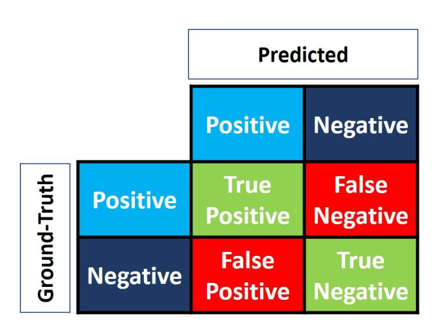
\includegraphics[width=0.8\linewidth]{pictures/Konfusionsmatrix_hs_analysis.png}
    \caption{Darstellung einer Konfusionsmatrix anhand von Annotationen (Ground-Truth) und Vorhersagen (Predicted) gemäß eines XNOR-Gatters}
    \label{fig:Konfusionsmatrix}
    \cite{noauthor_crc-modell_nodate}
\end{figure}

Precision
\begin{equation}
    Precision = \frac{\mbox{\textit{correctly classified actual positives}}}{\mbox{\textit{everything classified as positive}}} = \frac{TP}{TP + FP}
\end{equation}

Die Präzision beträgt im Idealfall ebenfalls 1,0 und hängt von der Anzahl falsch positiver Ergebnisse ab. Je geringer diese ist, desto besser die Genauigkeit. Präzision und Recall stehen sich in der Form gegenüber, als dass sie ein umgekehrtes Verhältnis haben und in der Regel mit steigender Präzision der Recall abnimmt und umgekehrt.

\begin{equation}
    Recall (\mbox{\textit{True Positive Rate, TPR}}) = \frac{\mbox{\textit{correctly classified actual positives}}}{\mbox{\textit{all actual positives}}} = \frac{TP}{TP + FN}
\end{equation}

Der Recall ist ein Indikator für die Erkennungswahrscheinlichkeit eines Modells, wobei ebenfalls ein Wert von 1,0 = 100\% angestrebt wird. Für die Anwendung an realen Datensätzen mit geringem Aufkommen positiver Ergebnisse bietet diese Berechnung mehr Aussagekraft als die Genauigkeit. Erfasst wird die Fähigkeit eines Modells zur richtigen Identifikation von positiven Instanzen.

\begin{equation}
    \mbox{\textit{FPR (False Positive Rate)}} = \frac{\mbox{\textit{incorrectly classified actual negatives}}}{\mbox{\textit{all actual negatives}}} = \frac{FP}{FP + TN}
\end{equation}

Die Wahrscheinlichkeit eines Fehlalarms, wie die Falsch-Positiv-Rate auch genannt wird, soll im Idealfall bei 0,0 und somit 0 \% liegen. Im Realfall ergibt sich die Aussagekraft aus der Anzahl von tatsächlichen Negativwerten und damit eine entsprechende Instabilität.

F1-Score
\begin{equation}
    2 * \frac{Precision * Recall}{Precision + Recall}
\end{equation}

Der F1-Score liefert den harmonischen Mittelwert anstelle des arithmetischen aufgrund der stärkeren Gewichtung von großen Unterschieden. Mit niedriger Precision oder Recall sinkt das Ergebnis selbst bei einem hohen Gegenwert, was ein schwerer zu manipulierendes Resultat bedeutet.

Accuracy
\begin{equation}
    Accuracy = \frac{\mbox{\textit{correct classifications}}}{\mbox{\textit{total classifications}}} = \frac{TP + TN}{TP + TN + FP + FN}
\end{equation}

Die Genauigkeit beschreibt den Anteil aller korrekten Klassifizierungen unabhängig von wahr oder falsch. Dies kann bei einer ausgewogenen Verteilung von TP und TN als eine ungefähre Übersicht für die Modellqualität dienen. Im Realfall liegen jedoch häufig unausgewogene Datensätze vor, bei denen entweder FN oder FP als Fehler überwiegt und damit die Aussagekraft reduziert. Entsprechend würde bei einem seltenen Aufkommen einer Klasse von nur 1\% das Modell in 100\% der Fälle \say{negativ} vorhersagen können, was in 99\% korrekt und dennoch nutzlos wäre.

Die Kürzel stehen für folgendes: TP = True Positive (wahre Positive), TN = True Negative (wahre Negative), FP = False Positive (falsche Positive) und FN = False Negative (falsche Negative).

Intersection over Union
\begin{equation}
    IoU = \frac{|A\cap B|}{|A\cup B|}
\end{equation}
Die Intersection over Union (zu Deutsch: Verhältnis der Schnittmenge zur Vereinigungsmenge, auch genannt Jaccard-Koeffizient) stellt ein Ähnlichkeitsmaß für Vektoren, Mengen und andere Objekte dar. Das dient der Beurteilung der Genauigkeit von Objekterkennungsmodellen und ihrer Optimierung. \cite{goodfellow_2016}

In der Form des Projekts stellt \textbf{IoU} die Schnittmenge der Ground-Truth-Pixelannotation und Vorhersage geteilt durch die Vereinigungsmenge derselben dar. Je ähnlicher Schnitt- und Vereinigungsmenge sind, desto mehr nähert sich der Wert eins an; bei vollständiger Übereinstimmung liegt er bei eins, bei keinerlei Übereinstimmung bei null. Die \textbf{mIoU} (\textbf{mean Intersection over Union}) beschreibt den durchschnittlichen IoU über mehrere Objekterkennungen zur besseren Gesamtakkuranz eines Modells. Da die Segmentierung pixelweise geschieht, ist der allgemeine Durchschnitt das geeignete Maß, solange das einzelne Objekt selbst keine Rolle spielt.

\textbf{Quantisierung/Optimierung für Edge-Geräte:} Um den Anspruch an die Rechenressourcen zu reduzieren, wird \textbf{Post Training Quantization (PTQ)} eingesetzt. Dabei wird die herkömmliche FP16-Aktivierungsausbreitung auf INT8 komprimiert, um den Speicherbedarf und die Inferenzlatenz auf dem Edge-Gerät zu senken. \textbf{Ergänzen}: Genauigkeitsverlust durch die Quantisierung anhand der obigen Metriken quantifizieren (FP16- vs. INT8-Modell). \cite{tensorflowPosttrainingQuantization}

